\documentclass[12pt]{article}
\usepackage{graphicx}
\usepackage{siunitx}
\usepackage{authblk}
\usepackage{amsmath}
\usepackage{booktabs} % for much better looking tables
\usepackage{array} % for better arrays (eg matrices) in maths
\usepackage{verbatim} % adds environment for commenting out blocks of text & for better verbatim
\usepackage{subfig} % make it possible to include more than one captioned figure/table in a single float
\usepackage{url}
\usepackage[parfill]{parskip}
\usepackage[top=1in, bottom=1in, left=0.9in, right=0.9in]{geometry}
\geometry{letterpaper}
\usepackage{mathptmx}
\usepackage{lineno}
\linenumbers
\usepackage[T1]{fontenc}
\usepackage{amsmath}
\numberwithin{equation}{section}
% \usepackage[numbers]{natbib}
% \usepackage{fancyvrb}
%\usepackage{lineno}
\usepackage{cleveref}
\usepackage{natbib}
\bibliographystyle{abbrvnat}
\setcitestyle{authoryear,open={(},close={)}}

\usepackage{pdflscape}
% \newcommand{\beginsupplement}{%
%         \setcounter{table}{0}
%         \renewcommand{\thetable}{S\arabic{table}}%
%         \setcounter{figure}{0}
%         \renewcommand{\thefigure}{S\arabic{figure}}%
%      }
    
\renewcommand{\thetable}{S\arabic{table}}%
\renewcommand{\thefigure}{S\arabic{figure}}%

\begin{document}
% \beginsupplement
\begin{landscape}
\begin{figure}
    \centering
    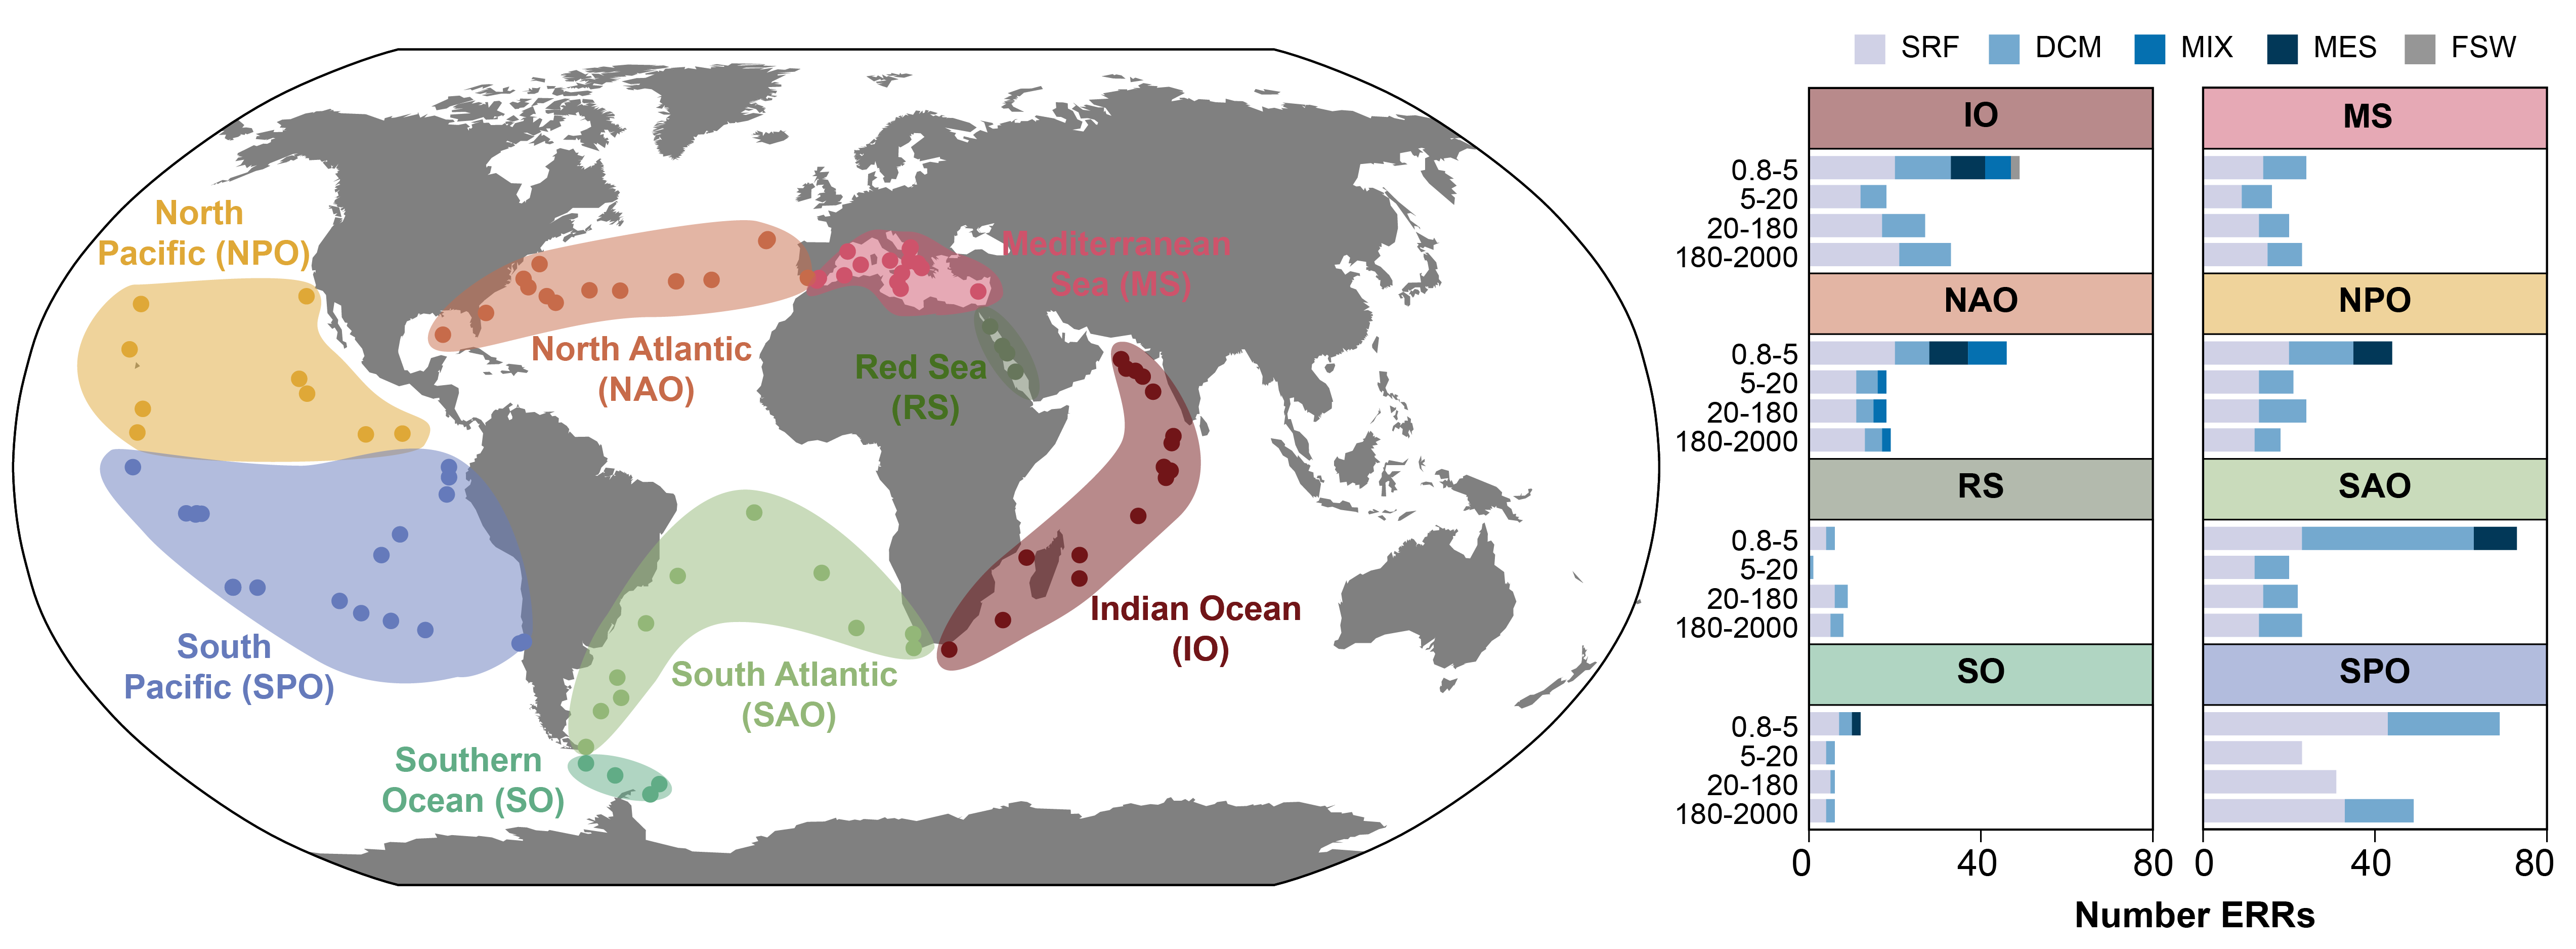
\includegraphics[width=0.95\columnwidth]{si-figures/Tara_stationMap-01.png}
    \caption{Sample Map thing.}
    \label{fig:tara-map}
\end{figure}
\end{landscape}



\begin{figure}
    \centering
    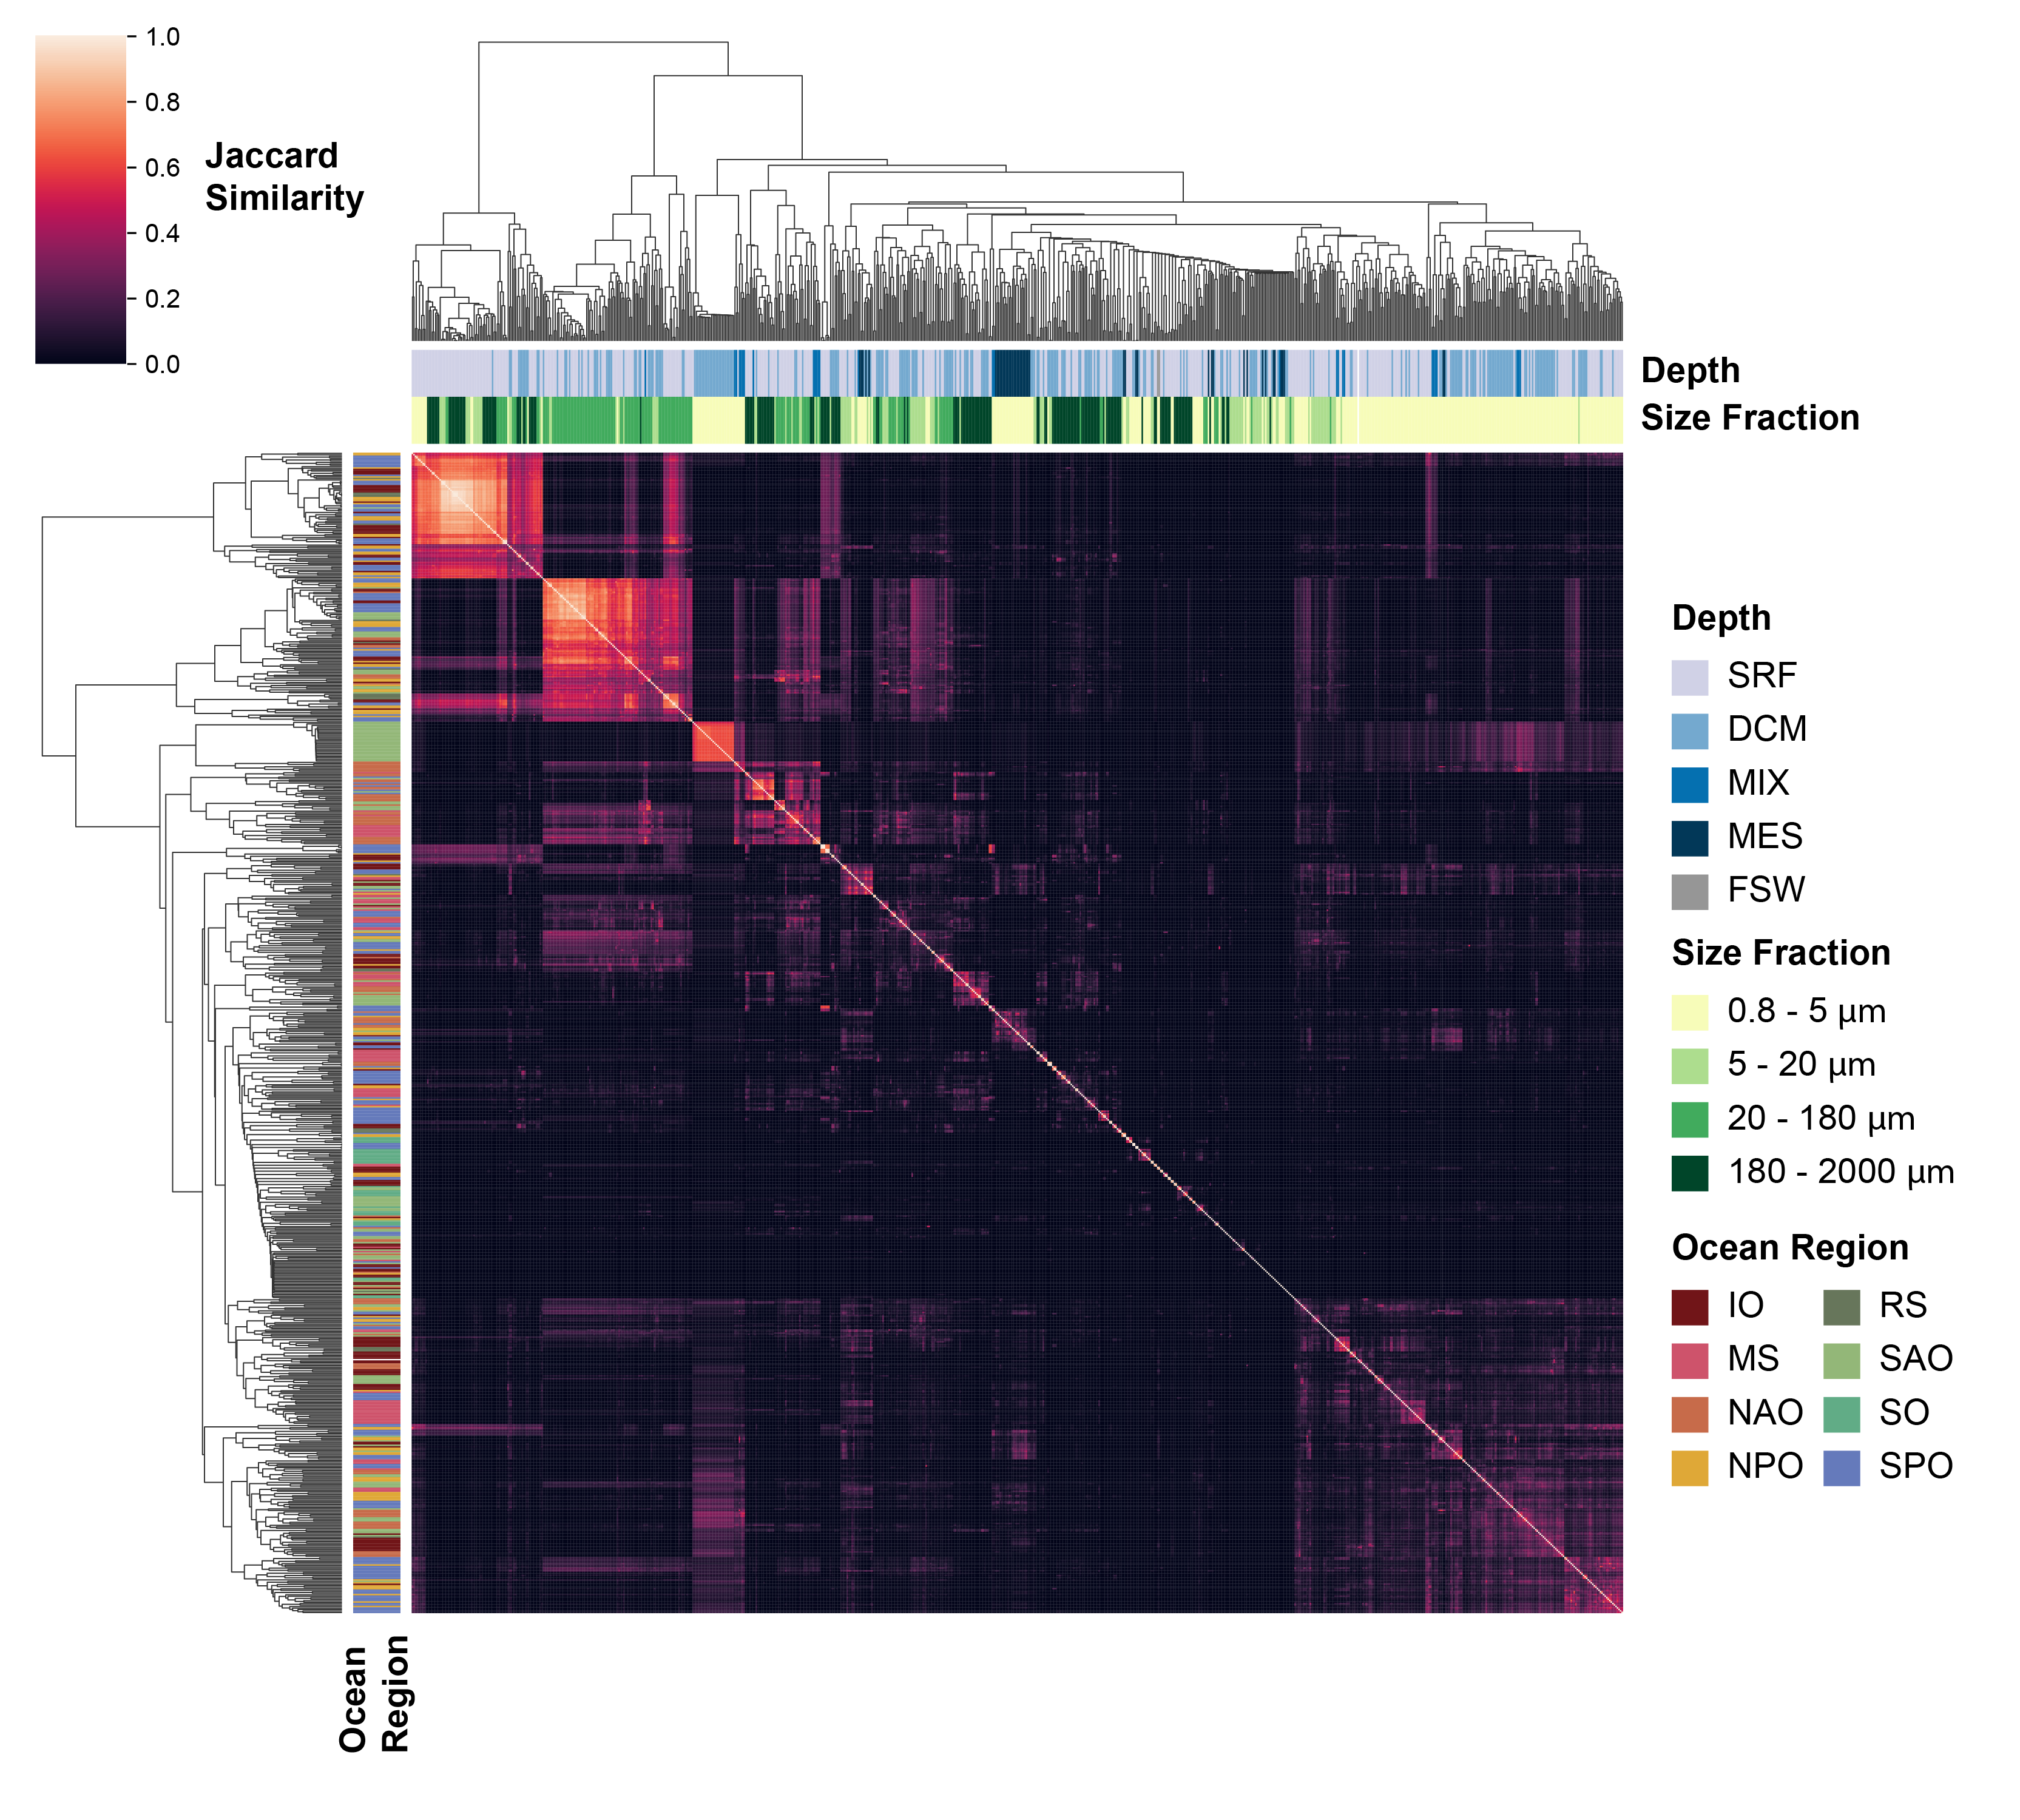
\includegraphics[width=0.95\columnwidth]{si-figures/modified-sourmash-region-size_depth-01.png}
    \caption{Sourmash comparison of all metagenomic samples from Tara large size fraction dataset. A minhash comparison was calculated using sourmash (k=31, scale=10,000) of the 824 metagenomic samples corresponding to the large size fraction metagenomic data from Tara (PRJEB4352). The relative sequence content similarity is shown as Jaccard similarity. Hierarchical clustering of samples based on sequence content is shown and sample identity (sample depth, size fraction, and ocean region) is highlighted by colored blocks.}
    \label{fig:sourmash}
\end{figure}


\begin{figure}
    \centering
    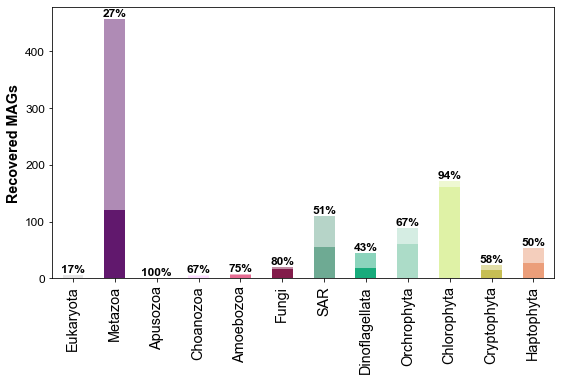
\includegraphics[width=0.9\columnwidth]{si-figures/MAGS_recovered.png}
    \caption{TOPAZ Recovered Eukaryotic MAGs. Course level taxonomic categorization of recovered eukaryotic TOPAZ MAGs (n=988). For each taxnomomic group, the total number of MAGs is depicted. MAGs within a taxonomic group that were highly complete ($>30\%$ BUSCO completeness) are shaded and the percentage of highly complete MAGs for each taxonomic group is reported. }
    \label{fig:recovered}
\end{figure}

\begin{landscape}
\begin{figure}
    \centering
    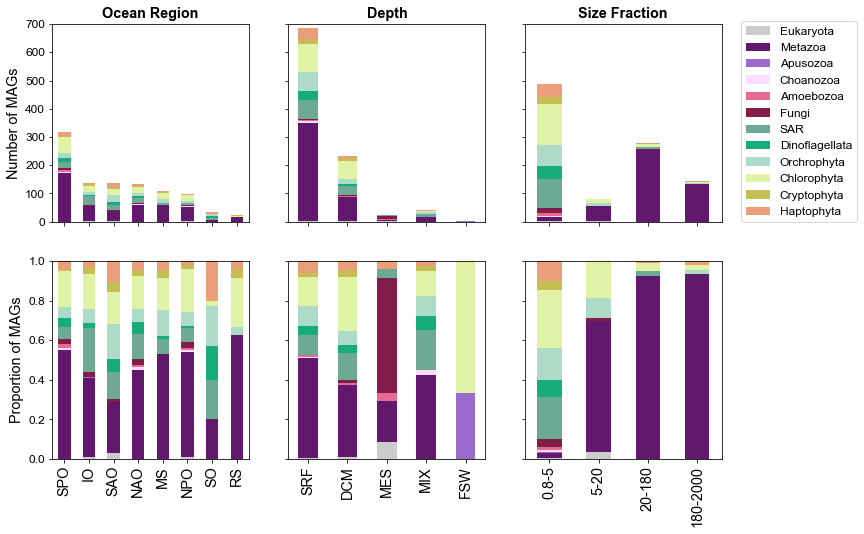
\includegraphics[width=0.95\columnwidth]{si-figures/ALL_MAG_distributions.png}
    \caption{TOPAZ Eukaryotic MAG as recovered by assembly group. The taxonomic breakdown of eukaryotic MAGs recovered within each general type of assembly group (based on Ocean Region, Depth, and Size Fraction) for all eukaryotic MAGs recovered in this study (n=988). Taxonomy is shown both as a total number recovered (top) and as a proportion of MAGs recovered for a given category (bottom). }
    \label{fig:all-dist}
\end{figure}
\end{landscape}

\begin{figure}
    \centering
    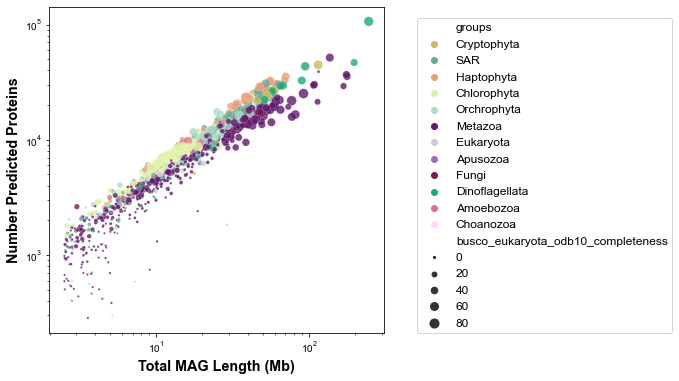
\includegraphics[width=0.95\columnwidth]{si-figures/ALL_MAGS_Num-Prot-Leng.png}
    \caption{The number of predicted proteins as a function of total MAG length.The number of predicted proteins for each eukaryotic TOPAZ mag (n=988) is plotted against the total MAG lenght (Mb). Each MAG is colored by its taxonomic group and the size of the circle is scaled by the estimated BUSCO completeness.}
    \label{fig:all-prot-len}
\end{figure}

\begin{landscape}
\begin{figure}
    \centering
    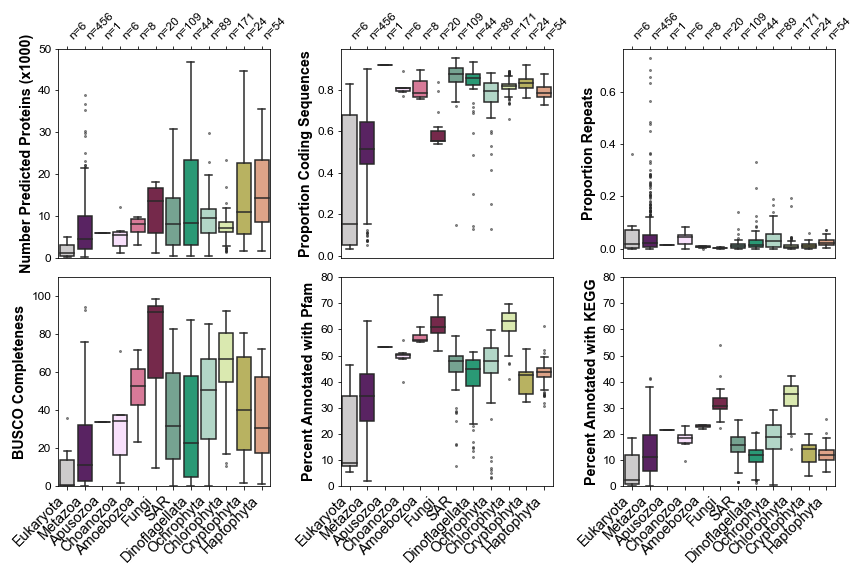
\includegraphics[width=0.8\columnwidth]{si-figures/ALL_MAG_protein_bar_plots.png}
    \caption{General completeness, protein predictions, and annotation of eukaryotic TOPAZ MAGs. The general characteristics of the predicted coding potential of all recovered TOPAZ eukaryotic MAGs is shown by general taxonomic group. ************}
    \label{fig:all-prot-bar}
\end{figure}
\end{landscape}

\begin{landscape}
\begin{figure}
    \centering
    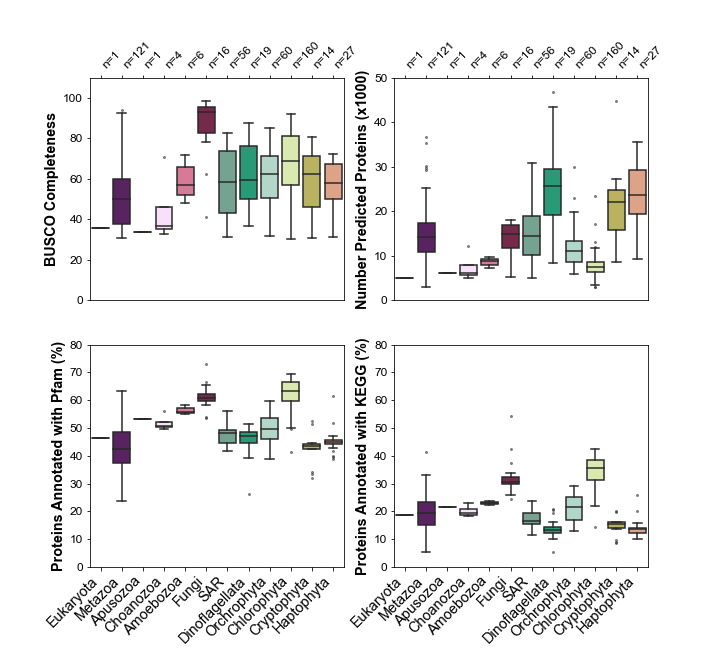
\includegraphics[width=0.8\columnwidth]{si-figures/HQ_MAG_protein_bar_plots.png}
    \caption{General completeness, protein predictions, and annotation of eukaryotic TOPAZ MAGs. The general characteristics of the predicted coding potential of all recovered TOPAZ eukaryotic MAGs is shown by general taxonomic group. ************}
    \label{fig:hq-prot-bar}
\end{figure}
\end{landscape}

\begin{landscape}
\begin{figure}
    \centering
    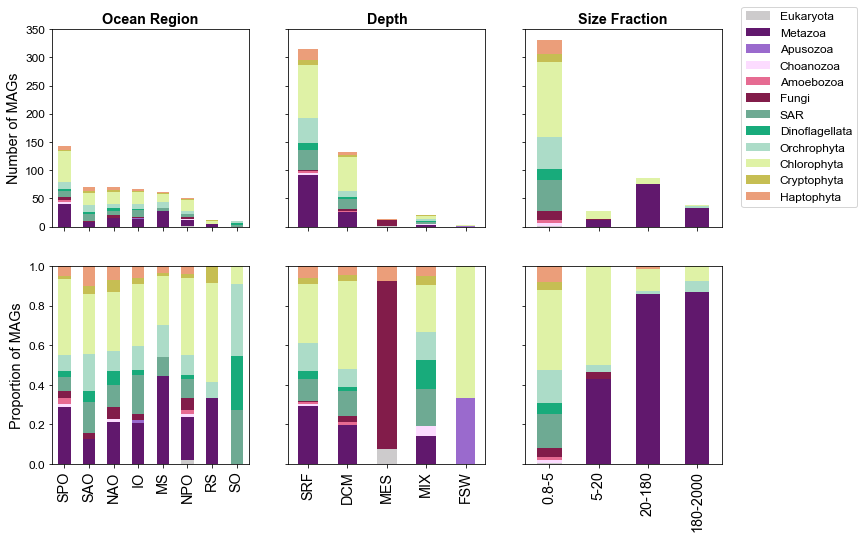
\includegraphics[width=0.95\columnwidth]{si-figures/HQ_MAG_distributions.png}
    \caption{TOPAZ Highly Complete Eukaryotic MAGs as recovered by assembly group. The taxonomic breakdown of eukaryotic MAGs recovered within each general type of assembly group (based on Ocean Region, Depth, and Size Fraction) for highly complete eukaryotic MAGs ($>30\%$ BUSCO completeness)recovered in this study (n=485)). Taxonomy is shown both as a total number recovered (top) and as a proportion of MAGs recovered for a given category (bottom). }
    \label{fig:hq-dist}
\end{figure}
\end{landscape}


\begin{figure}
    \centering
    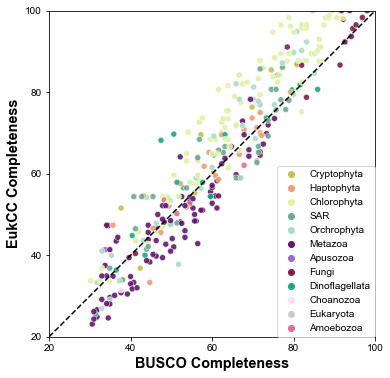
\includegraphics[width=0.8\columnwidth]{si-figures/HQ_BUSCO-EukCC-comp.png}
    \caption{Estimated completeness of eukaryotic MAGs using eukaryotic BUSCO gene set and eukcc.  }
    \label{fig:eukcc}
\end{figure}


\begin{landscape}
\begin{figure}
    \centering
    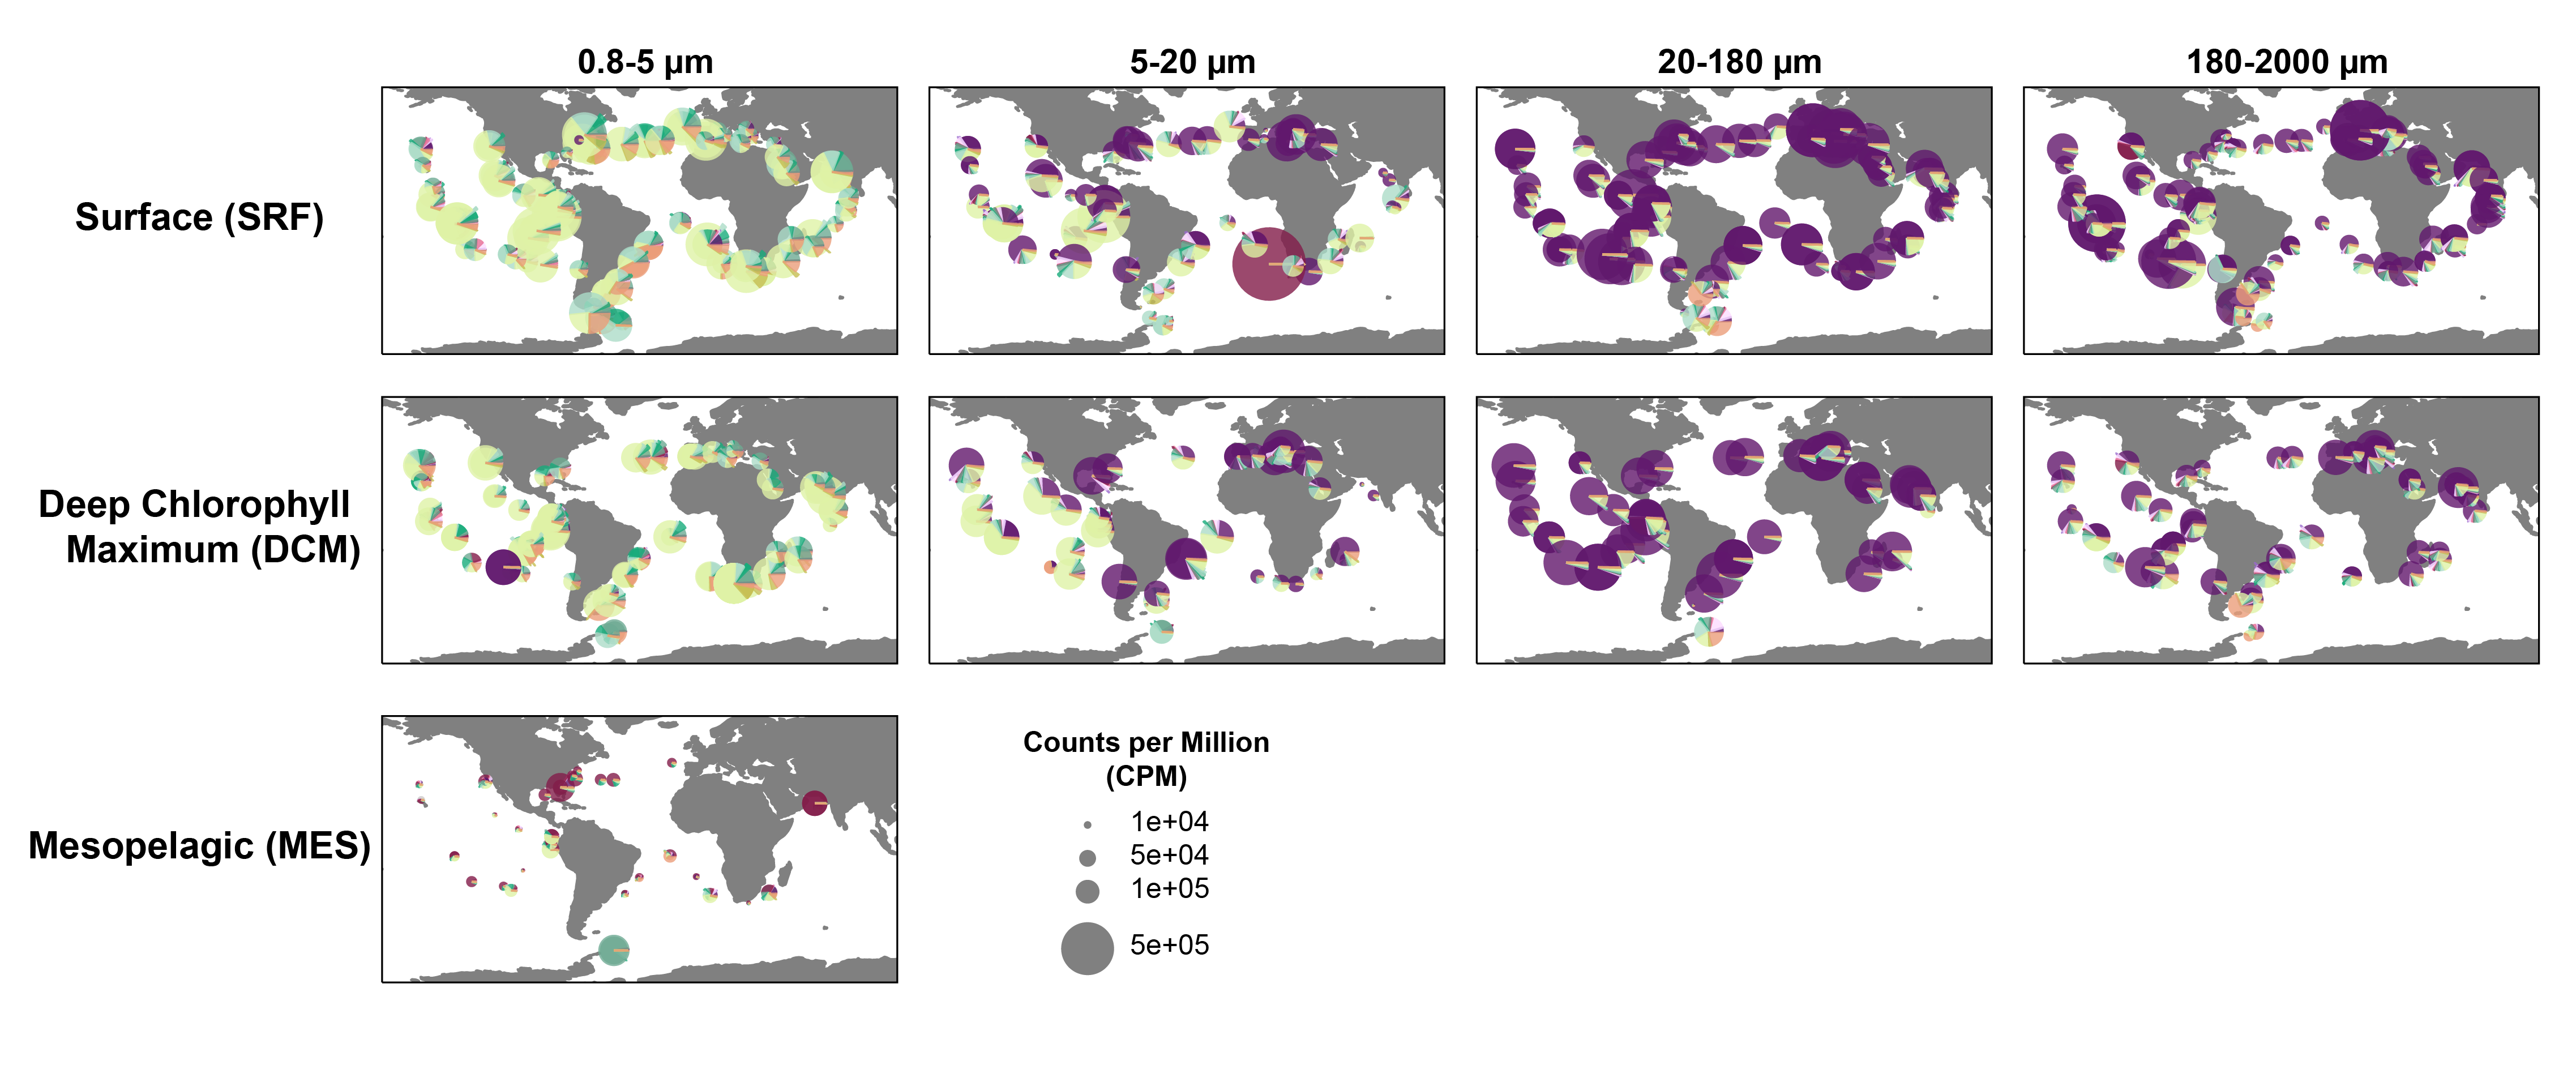
\includegraphics[width=0.95\columnwidth]{si-figures/Distribution-Map-Taxonomy-01.png}
    \caption{ }
    \label{fig:map}
\end{figure}
\end{landscape}

\begin{figure}
    \centering
    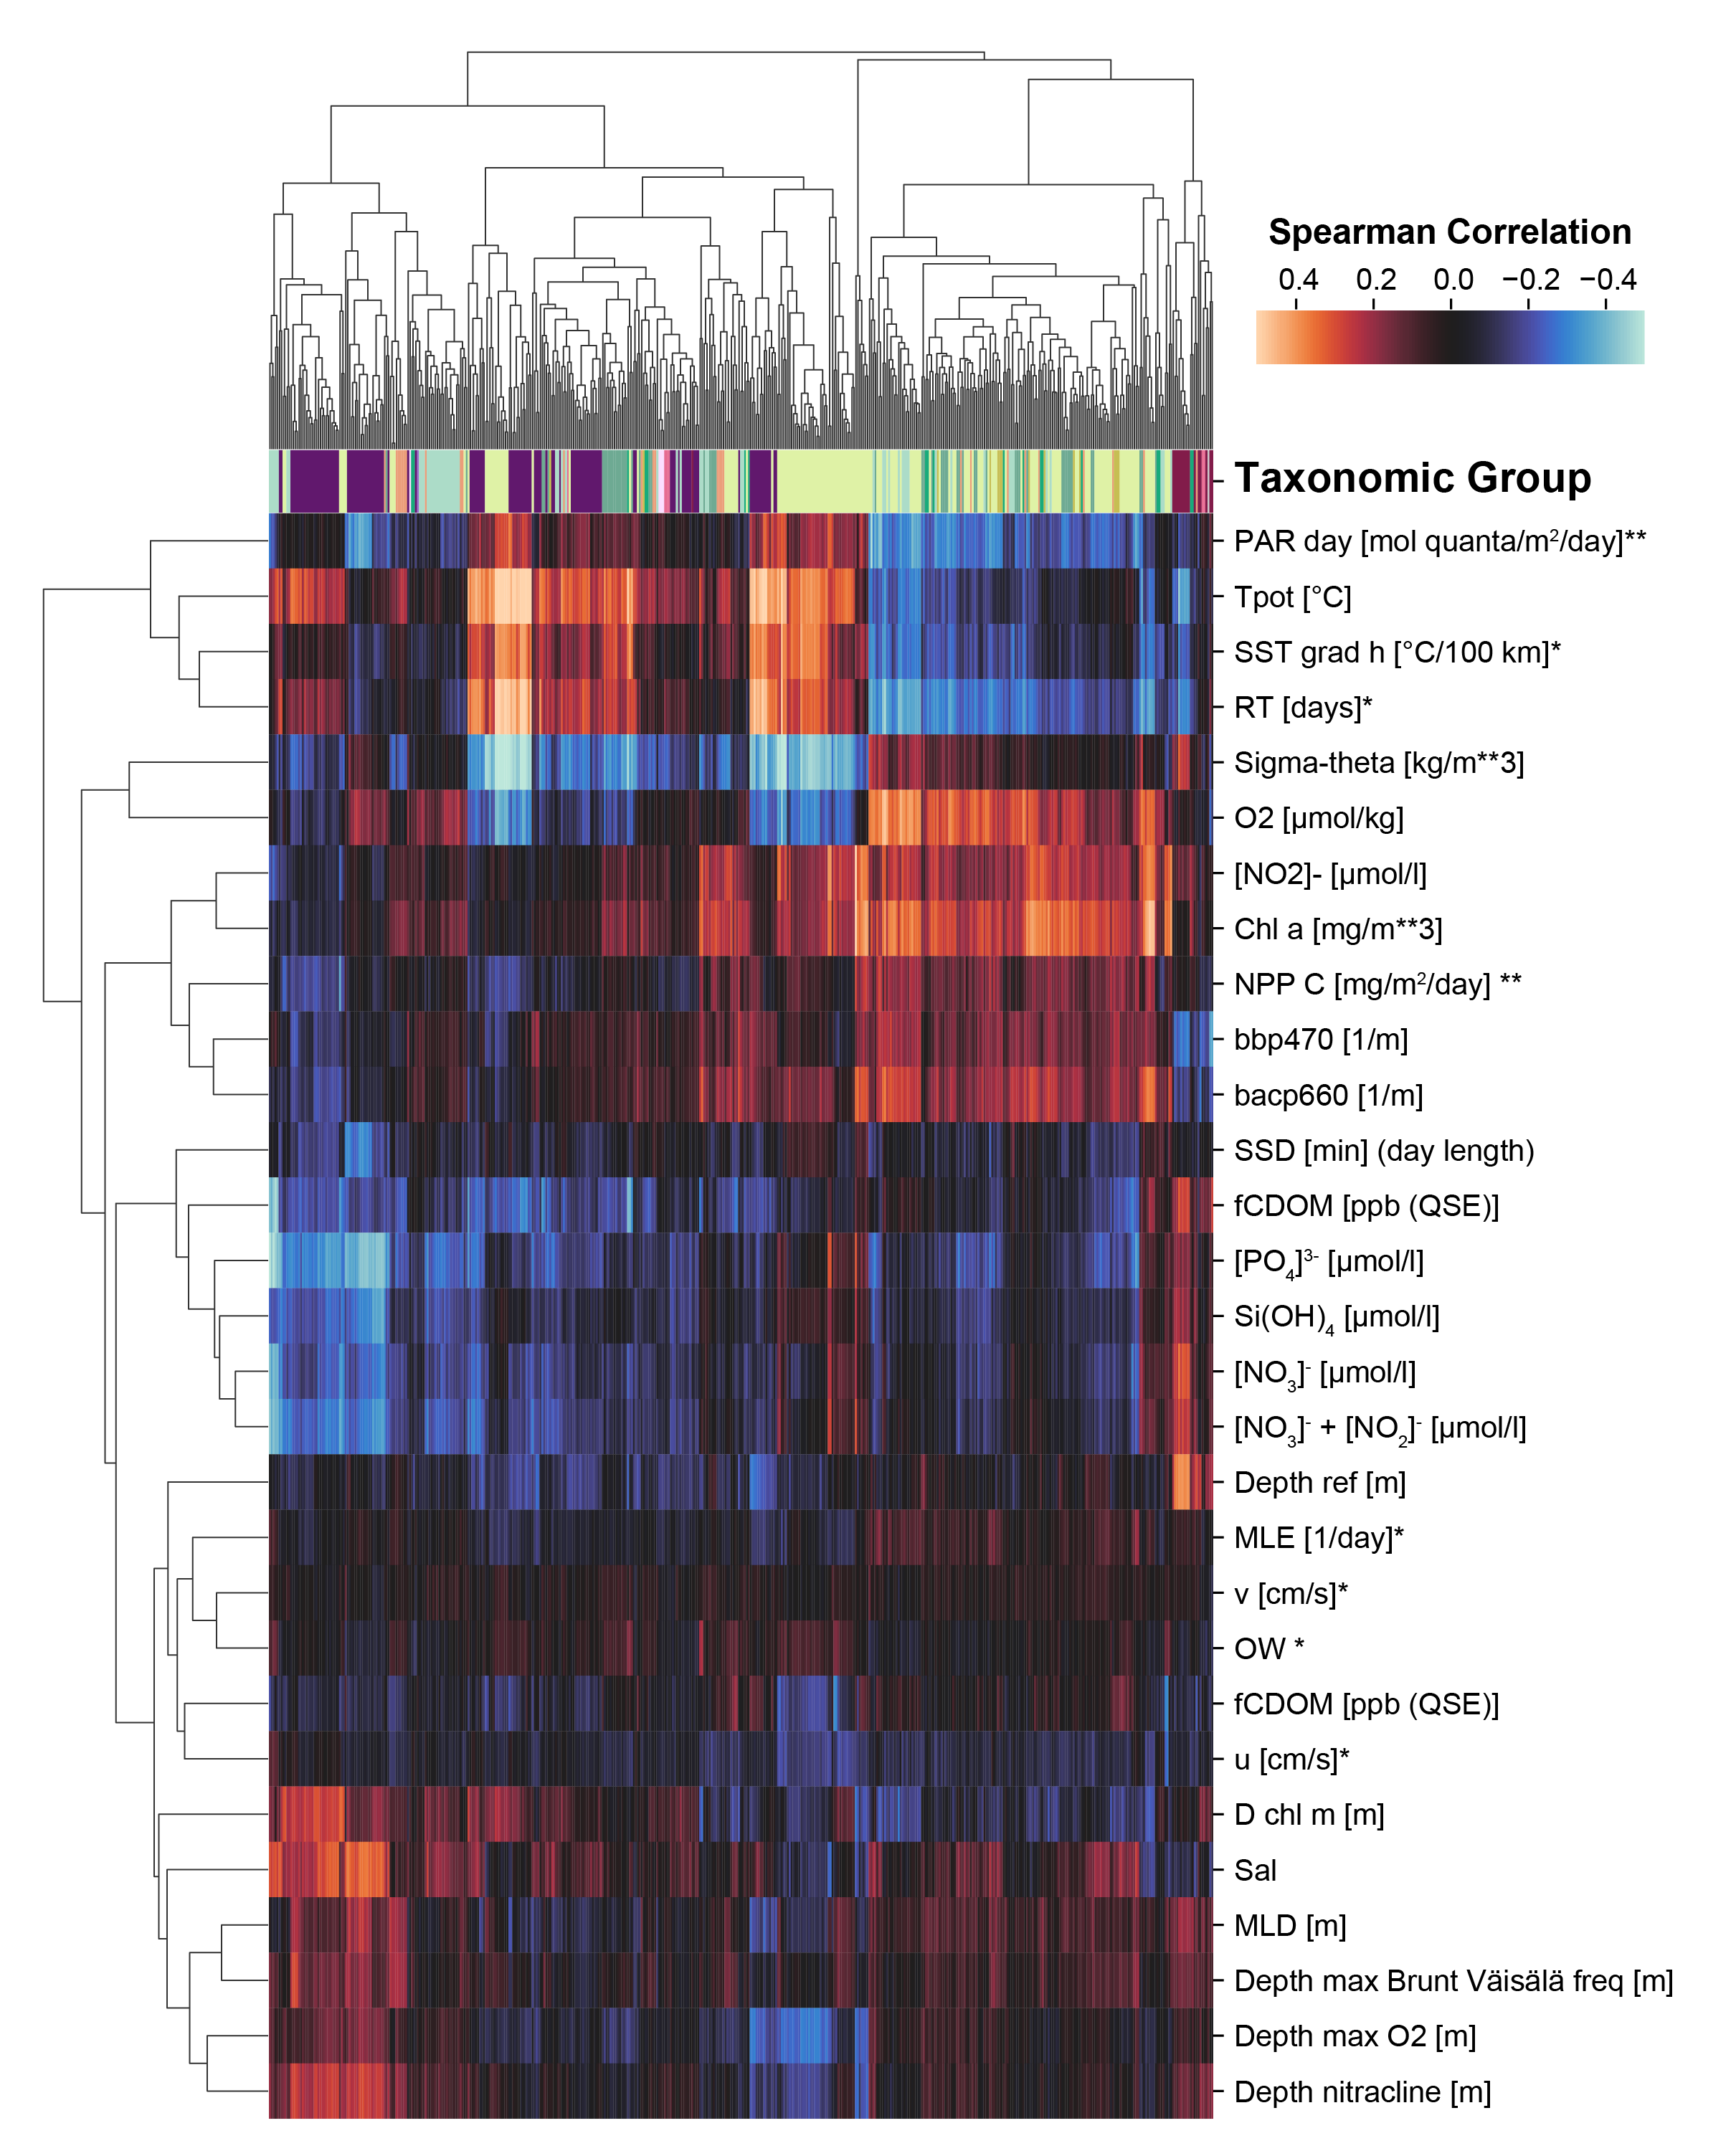
\includegraphics[width=0.9\columnwidth]{si-figures/modified-individual-mag-group-correlation-01.png}
    \caption{ }
    \label{fig:ind-corr}
\end{figure}


\begin{figure}
    \centering
    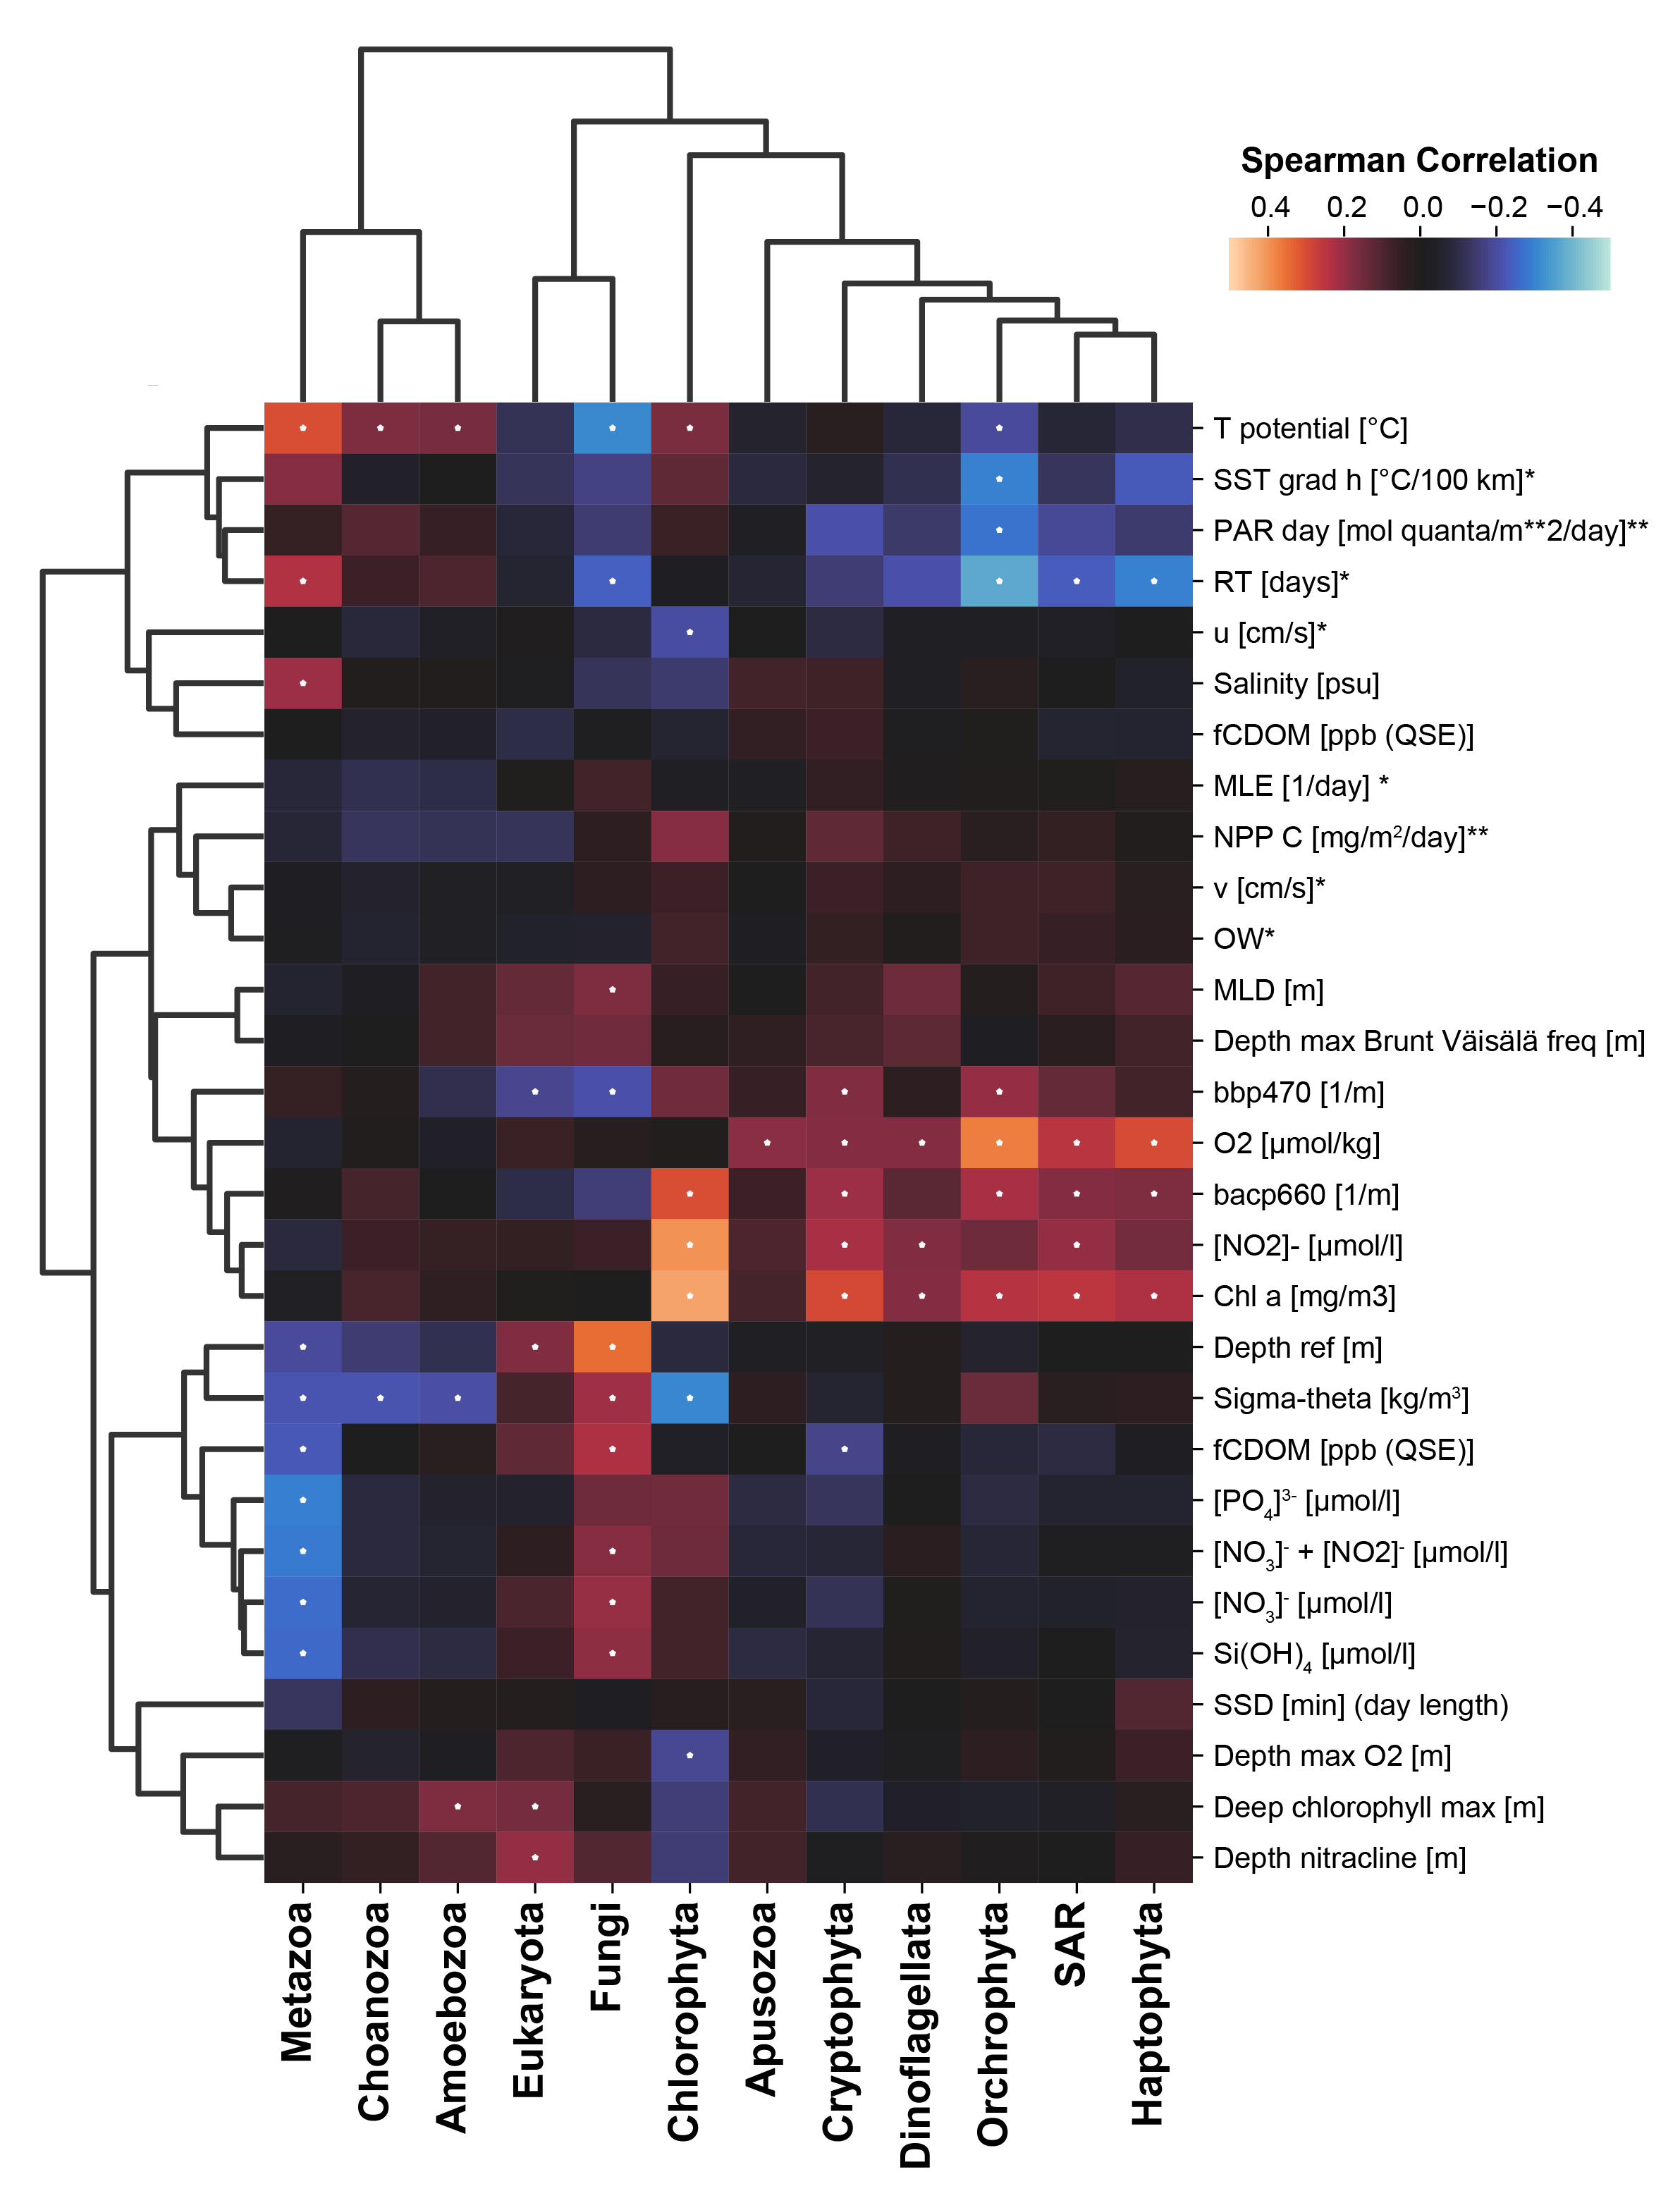
\includegraphics[width=0.9\columnwidth]{si-figures/mag-group-correlation-01.png}
    \caption{ }
    \label{fig:env-corr}
\end{figure}


\end{document}
